%!TEX root = ../dissertation.tex
\begin{savequote}[75mm]
Noli turbare circulos meos
\qauthor{Archimedes}
\end{savequote}

\chapter{The Large Hadron Collider and the ATLAS Detector}
Look at \cite{run1note}, \cite{jinstpaper}

\newthought{The CERN accelerator complex and its experiments} stand as a testament to human ingenuity and

\section{The CERN Accelerator Complex}
\begin{itemize}
\item ionize hydrogen in $\vector{E}$
\item LINAC 2: 50 MeV
\item BOOSTER: 1 GeV
\item PS: 26 GeV
\item SPS: 450 GeV
\item LHC
\end{itemize}

\begin{figure}[!htbp]\captionsetup{justification=centering}
  \centering
  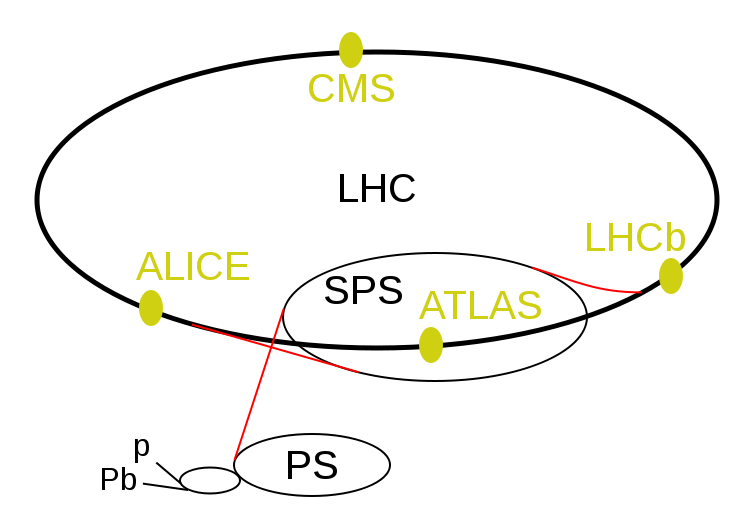
\includegraphics[width=0.800000\linewidth]{figures/atlas/lhc}
  \caption{The Large Hadron Collider.}
  \label{fig:cern}
\end{figure}

\section{The Large Hadron Collider}
The Large Hadron Collider
\afterpage{\begin{landscape}
\begin{figure}[!htbp]\captionsetup{justification=centering}
  \centering
  \begin{subfigure}[t]{0.4950000\linewidth}\centering\includegraphics[width=\textwidth]{figures/atlas/lhcschematic}}\caption{}\end{subfigure}
  \begin{subfigure}[t]{0.4950000\linewidth}\centering\includegraphics[width=\textwidth]{figures/atlas/fig_LHC_area_overview}}\caption{}\end{subfigure}
  \caption{Schematic and detailed views of the LHC ring. IC: \cite{lhccartoon}, \cite{lhcdetail}}
  \label{fig:lhcring}
\end{figure}
\end{landscape}}

Describe the magnets I guess

\section{The ATLAS Coordinate System}
{\bf A} {\bf T}oroidal {\bf L}HC {\bf A}pparatu{\bf S} is one of the two general purpose, high luminosity detectors at the LHC, located at Interaction Point 1, as described above.  With a length of 44 m and a height of 25 m, it is the detector with largest physical dimensions at the LHC.\footnote{This is the only reason CMS can call itself ``compact.''}.  The ATLAS detector and its main components are shown in Figure \ref{fig:atlas}

\begin{figure}[!htbp]\captionsetup{justification=centering}
  \centering
  \includegraphics[width=0.8\linewidth]{figures/atlas/atlasfullp}
  \caption{The ATLAS detevtor with principal subsystems shown.}
  \label{fig:atlas}
\end{figure}

While primarily a high luminosity proton-proton collision detector, ATLAS does collect heavy ion collision data, typically for one month during a year of typical operation.  

The ATLAS coordinate system is cylindrical and shown in Figure

\begin{figure}[!htbp]\captionsetup{justification=centering}
  \centering
  \includegraphics[width=0.800000\linewidth]{figures/coord}
  \caption{The  ATLAS coordinate system.}
  \label{fig:acoord}
\end{figure}
\begin{description}
\item[(Pseudo)Rapidity] Rapidity $y=\frac{1}{2}\ln\left[\frac{E+p_z}{E-p_z}\right]$, pseudorapidity $\eta=-\ln\tan\frac{\theta}{2}$; same for massless particles
\item[$\phi$,$r$] Azimuthal angle and perpendicular distance from beam axis
\item[$p_T,E_T,E^{miss}_T$] Transverse momentum ($p_T=\sqrt{p_x^2+p_y^2}$), transverse energy, and missing transverse energy ($E_T=\sqrt{E_x^2+E_y^2}=-E_T^{miss}$).  Neutrinos only show up as $E_T^{miss}$.
\item[Barrel] Lower $\left|\eta\right|$ material; cylindrical layers of the detector
\item[End Cap] Higher $\left|\eta\right|$ material; arranged in disks centered on the beam pipe
\end{description}


\section{The Inner Detector}
The inner detector uses two layers of silicon detector and one layer of gas straw detectors with filaments for $e/\pi$ discrimination.  There's a 2T magnetic field generated by a superconducting solenoid surrounding the ID (4.5 K).  The ID's extent is to $\left|\eta\right|<2.5$.  Generally, there are two radiation lengths in the inner detector (it varies with $\eta$). So let's describe the sub-systems:
\begin{figure}[!htbp]\captionsetup{justification=centering}
  \centering
  \includegraphics[width=0.800000\linewidth]{figures/atlas/ind_det_labp}
  \caption{The ATLAS inner detector.}
  \label{fig:indet}
\end{figure}
\subsection{The Pixel Detector}
\begin{itemize}
\item Cooled to $\sim-5$\celsius\  with $N_2$ gas, 150--600 V
\item 10(115) $\mu$m resolution in $r-\phi$ ($z$); pixels are $50\times400(600)\times250$ $\mu$m
\item Barrel: Layers at 50.5, 88.5, and 122.5 mm at a 20\degree\ tilt with overlap in $r-\phi$
\item End Cap: 495, 580, 650 mm; rotate in $\phi$ by 3.75\degree\
\end{itemize}
\subsection{The Silicon Microstrip Detector (SCT)}
\begin{itemize}
\item Cooled to $\sim-5$\celsius\  with N$_2$ gas, 150--600 V
\item 17(580) $\mu$m resolution in $r-\phi$ ($z$)
\item Barrel: 11\degree\ tilt, 4 layers (299, 371, 443, 514 mm), rectangles
\item End Cap: 9 disks each side (934--2720 mm), trapezoids
\end{itemize}
\subsection{Transition Radiation Tracker (TRT)}
(Transition radiation is the X-ray emission from relativistic electrons as they go from dielectric to gas.)
\begin{itemize}
\item $\left|\eta\right|<2$; 130 $\mu$m resolution; Straws 4 mm diameter; Xe-CO$_2$-O$_2$ (70-27-3); $-1500$ V
\item Filaments/foil cause the transition radiation for $e/\pi$ identification $-dE/dx\sim\gamma$
\item Barrel: 73 layers, 144 cm long, along $z$
\item End Cap: 160 cm, 37 cm long, disks, each straw points in $\hat{r}$ at constant $\phi$
\end{itemize}


\section{The ATLAS Calorimeters}
\subsection{Calorimeter Resolution}
Following Tully's notation, we parameterize the momentum resolution of a \emph{tracker} as:
\begin{equation}
\frac{\sigma_{p_T}}{p_T}=c_0\oplus c_1\cdot p_T
\label{eqn:ptres}
\end{equation}
Effects: \emph{multiple scattering}: $c_0=0.5-2\%$ (much of a problem at high $B$); \emph{curvature resolution} $c_1=10^{-3}-10^{-4}$ GeV$^{-1}$ (related: charge confusion happens when high $p_T$ tracks have small curvature, wrong sign)

\begin{equation}
\frac{\sigma_E}{E}=\frac{S}{\sqrt{E}}\oplus\frac{N}{E}\oplus C
\label{eqn:eres}
\end{equation}
$S\sim2.7\%\sqrt{d_{active}\left[\text{mm}\right]/f_{samp}}$ (the stocastic term; the sampling fraction in the tile calorimeter is $\sim1/36$) and $C$ (constant term, calibration effects---would be zero for a single detector because you could understand it ``perfectly'' in principle) will be noted for different calorimeters below.  $N\sim0.1-0.5$ GeV.

Calorimeter energy resolution is noted in Eqn. \ref{eqn:eres}. 89 K, liquid nitrogen, similar readouts.
\begin{figure}[!htbp]\captionsetup{justification=centering}
  \centering
  \includegraphics[width=0.800000\linewidth]{figures/atlas/ehfcalp}
  \caption{The ATLAS calorimeters.}
  \label{fig:indet}
\end{figure}

\subsection{The Electromagnetic Calorimeter (ECAL)}
\begin{itemize}
\item $S=0.1$ GeV$^{-1/2}$, $C=0.002$;450 ns drift time
\item 2-4 interaction lengths, $20-40X_0$, LAr/Pb active/absorber
\item accordion geometry, absorber thickness 1.53 (1.13) mm $\left|\eta\right|<(>)0.8$ (constant $f_{samp}$
\item Pre-sampler: $\left|\eta\right|<1.8$ 11 mm of LAr (in barrel)
\item Barrel: $\left|\eta\right|<1.475\right|$, 3 layers: 1150, 1250, 2050 mm
\item End Cap: $1.375<\left|\eta\right|<2.5(3.2)\right|$ inner (outer) wheel, 3 (2) layers: out to 3100 mm
\end{itemize}
\subsection{The Hadronic Calorimeter (HCAL)}
\begin{itemize}
\item $S=0.5$ GeV$^{-1/2}$, $C=0.05$ (0.03 after calibration)
\item $\sim10$ interaction lengths (up to 20), 2.28--4.25 m
\item $0.1\times0.1 (0.2\times0.2)$ $\eta,\phi$ granularity with(out) tracking
\item Barrel: polystyrene/steel, staggered matrix, $\left|\eta\right|<1.7$ (UV scint.), 1800 V, 400 ns DT
\item End Cap: $1.5<\left|\eta\right|<3.2\right|$ LAr/Cu; two wheels each side $372(475)-2030$ mm $r$, $4300<z<6100$ mm
\end{itemize}
\subsection{The Forward Calorimeter (FCAL)}
\begin{itemize}
\item $S\approx1$ GeV$^{-1/2}$
\item $3.1<\left|\eta\right|<4.9$; LAr/Cu-W, matrix of absorber, rods inside tubes (LAr lives in the gap between the rod and tube)
\end{itemize}


\section{The Muon Spectrometer}
\begin{figure}[!htbp]\captionsetup{justification=centering}
  \centering
  \includegraphics[width=0.800000\linewidth]{figures/atlas/muonspecp}
  \caption{The ATLAS muon spectrometer.}
  \label{fig:ms}
\end{figure}
\begin{itemize}
\item Three layers: 5, 7.5, 10 m (barrel); 7, (11, small layer EC toroid), 13, 21 m (end cap)
\item Air toroid 4.5 K LHe, 4 T max (0.5--1.0 T), coils. 20.5 kA
\item momentum resolution, charge reconstruction: 5 GeV up to 3 TeV (10\% resolution at 1 TeV (3\% at 100 GeV)) 
\end{itemize}
\subsection{Precision Detectors}
\begin{itemize}
\item MDT: 3 cm diameter Monitored Drift Tubes, Ar/CO$_2$ gas, W-Re wire at 3 kV, $\left|\eta\right|<2.0$, 700 ns DT
\item CSC: Cathode Strip Chamber, $2.0\left|\eta\right|<2.7$,  multiwire proportional chamber, more radiation hard, DT $\lesssim40$ ns
\end{itemize}
\subsection{Trigger Detectors}
\begin{itemize}
\item $\left|\eta\right|< 2.4$, must be fast, approx. $p_T$ and pos. of $\mu$ track
\item RPC: Resistive Plate Chamber, parallel plate detector, 2 mm, 9.8 kV, 5 ns; 3 layers, barrel
\item TGC: Thin Gap Chamber, multiwire proportional chamber, DT+prop. $<25$ ns; 4 layers, EC
\end{itemize}


